\chapter{Design Motivation}
\label{ch:fddp-design}

%%%%%%%%%%%%%%%%%%%%%%%%%%%%%%%%%%%%%%%%%%%%%%%%%%%%%%%%%%%%%%%%%%%%
%\section{Introduction to Dual-Phase Far Detector in DUNE}
\section{Introduction to the DUNE \dual Far Detector Design}
\label{sec:fddp-design-highlight}

%Similarly as for the \single design the \dword{dpmod} is aiming at opening new windows of opportunity in the studyof neutrinos.  DUNE's rich physics program, with discovery potential for \dword{cp} in the neutrino sector, and its capability to make significant observations of nucleon decay and astrophysical events, is enabled by the exquisite resolution of the \lartpc detector technique which is further augmented in the \dual design. The \dual design allows for improving the \dword{s/n} ratio in the charge readout and lowering thresholds for the smallest observable signals while achieving at the same time a finer readout granularity.  The \dual technology aims to build larger drift volumes, thereby reducing %%so 
%the presence of dead materials in the \lar target. The basic physics requirements are identical for both the \single and \dual designs, %%with 
%however, some aspects of the \dual design offer augmented performance. % under some aspects.

Similarly to the \single design, the \dword{dpmod} aims to open new windows of opportunity in the study
of neutrinos.  DUNE's rich physics program, with discovery potential for \dword{cp} in the neutrino sector, and its capability to make significant observations of nucleon decay and astrophysical events, is enabled by the exquisite resolution of the \lartpc detector technique, which the \dual design further augments. This design improves the \dword{s/n} ratio in the charge readout,  lowering the threshold for the smallest observable signals while also achieving a finer readout granularity.  The \dual technology enables the construction of larger drift volumes, thereby reducing %so 
the quantity of nonactive materials in the \lar. Although the physics requirements are identical for both the \single and \dual designs, %with 
 some aspects of the \dual design offer augmented performance. % under some aspects.

%%%%%%%%%%%%%%%%%%%%%%%%%%%%%%%%%%%%%%%%%%%%%%%%%%%%%%%%%%%%%%%%%%%%

\section{\dual \lartpc Operational Principle}
\label{sec:fddp-operational-principle}

%The basic operational principle is very similar to that of the \single design. %as for the Single-phase design. 
%The precision tracking and calorimetry offered by the \dual
%technology provides excellent capabilities for identifying interactions of interest while mitigating sources of background.  Charged particles traversing the active volume of the \lartpc ionize the medium, while also producing scintillation light.  The ionization \fixme{electron? or charge?} drifts along an \efield that is present throughout the volume, towards a segmented anode.

The basic operational principle is very similar to that of the \single design. 
Charged particles that traverse the active volume of the \lartpc ionize the medium, while also producing scintillation light.  The ionization electrons drifts along an \efield towards a segmented anode where they deposit their charge, and \dwords{pd} pick up the scintillation light.
The precision tracking and calorimetry offered by the \dual
technology provides excellent capabilities for identifying interactions of interest while mitigating sources of background.  
Whereas the \single design has multiple drift volumes, the \dword{dpmod} design allows for a single, fully homogeneous \lar volume with a much longer drift length. This volume is surrounded by a \dword{fc} on the sides and a cathode at the bottom, which together define the drift field. 

%The key concept of the \dual design relies on the possibility of amplifying the ionization signal in avalanche processes. In the \single design charges are drifted horizontally to the anode, which consists of a set of induction and collection wire layers immersed in the \lar. In the \dual design electrons are drifted vertically towards an extraction grid just below the liquid-vapor interface. After reaching the grid, the electrons are extracted from the liquid to the gas phase due to an \efield stronger than the drift field. Once in the gas, electrons can be amplified in avalanches that occur in the high-field regions present within micro-pattern gas detectors, the \dwords{lem}. The amplified electrons are then eventually collected on a finely segmented anode with two perpendicular collection views. 

The key differentiating concept of the \dual design is the amplification of the ionization signal in \textit{avalanche} processes. In the \single design, charges drift horizontally to the anode, which consists of a set of induction and collection wire layers immersed in the \lar. In the \dual design, electrons drift vertically upward towards an extraction grid just below the liquid-vapor interface. After reaching the grid, an \efield stronger than the drift field extracts the electrons from the liquid up into the gas phase. Once in the gas, electrons encounter micro-pattern gas detectors with high-field regions, called \dwords{lem}. The \dwords{lem} amplify the electrons in avalanches that occur in these high-field regions. %The amplified electrons are then collected on a finely segmented anode with two perpendicular collection views. 
The amplified charge is then collected and recorded on a \twod anode
consisting of two sets of \SI{3.125}{mm}-pitch gold-plated copper strips that provide the $x$
and $y$ coordinates (and thus two views) of an event.

%The \dword{dpmod} design allows for  %foresees  a single, fully homogeneous \lar volume with a long drift length. This volume is surrounded (sides and bottom) by a \dword{fc} and a cathode, which together define the drift field. 

%At the top of the \dword{dpmod}, an anode, consisting of a set of active detector elements called \dwords{crp}, sits above the liquid, in the gas phase. The \dwords{crp} integrate the \dwords{lem} and anodes, and support the extraction grid, which is immersed in the liquid. They can be individually positioned at a few millimeters parallel to the interface between the liquid and the gas, ensuring that the extraction grid is immersed.
%The extraction grid, \dword{lem} and anode are assembled into three-layered \textit{sandwiches} with precisely defined inter-stage distances and inter-alignment,  which are then connected together horizontally into

The extraction grid, \dword{lem} and anode are assembled into three-layered \textit{sandwiches} 
with precisely defined inter-stage distances and inter-alignment,  which are then connected together horizontally into
modular units of area \num{9}~m$^2$. These units are called \dwords{crp}.
The \dwords{crp} integrate the \dwords{lem} and anodes, and support the extraction grid. These units can be individually positioned in a horizontal plane a few millimeters beneath the liquid-gas interface, ensuring complete immersion of the extraction grid.


The argon scintillation light, which at a wavelength of  \SI{128}{nm} is deep in the UV spectrum and it is recorded by an array of \dwords{pmt} located below the cathode. %The \dwords{pmt} are coated with a material that shifts the wavelength closer to the visible spectrum and subsequently record the time and pulse characteristics of the incident light.

The \dwords{pmt}, coated with a wavelength-shifting material, shifts the light  closer to the visible spectrum and records the time and pulse characteristics of the incident light.

%The performance of the  \lartpc hinges on several key factors.  First, the purity of the \lar must be extremely high in order to allow the ionization to be able  to drift over several meters towards the anode planes.  The levels of electronegative contaminants (e.g., oxygen, water), must be reduced andmaintained to $\sim$ppt levels in order to achieve minimum charge attenuation over the longest drift lengths in the \lartpc.  The \dual and \single designs are subject to the same purity requirements. Second, the electronic readoutof the \lartpc requires very low noise levels so that the signal from the drifting ionization  is clearly discernible over the baseline of the electronics.  %%The \dual design relies on the same purity requirements as for Single-Phase and on the use of low noise cryogenic electronics. However the impact of these aspects on the performance is mitigated by the possibility of amplifying the electrons signal in the gas phase. On the other hand the \dual design requires higher voltages to be applied to the cathode in order to define the drift field over longer paths.
%This requires use of low-noise cryogenic electronics. However the impact of these aspects on the performance is mitigated by the possibility of amplifying the electrons signal in the gas phase. On the other hand the \dual design requires higher voltages to be applied to the cathode in order to define the drift field over longer paths.

Two key factors affect the performance of the  \lartpc{}.  First, the \lar purity must be extremely high in order to achieve minimum charge attenuation over the longest drift lengths in the \lartpc{}.  This requires that the levels of electronegative contaminants (e.g., oxygen, water), be reduced and
maintained at $\sim$ppt levels.  The \dual and \single designs are subject to the same purity requirements. 
%
Second, the electronic readout
of the \lartpc{} requires very low noise levels in order that the signal from the drifting electrons
%\fixme{charge} 
be clearly discernible over the baseline of the electronics.  This requires use of low-noise cryogenic electronics. 

The amplification of the electron signal in the gas phase mitigates the potential impact of these factors on the performance of the \dual design.  On the other hand this design requires  higher voltages on the cathode, relative to the \single, due to the longer drift field. 


\begin{dunefigure}[Principle of the \dual readout]{fig:figure-label-DPprinciple}{Principle of the \dual readout}
%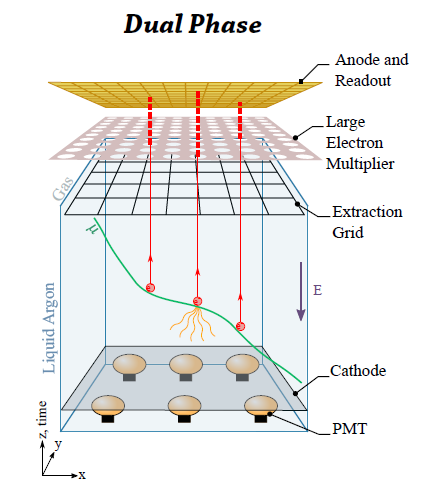
\includegraphics[width=0.6\textwidth]{dualphase-principle}
\end{dunefigure}

%%%%%%%%%%%%%%%%%%%%%%%%%%%%%%%%%%%%%%%%%%%%%%%%%%%%%%%%%%%%%%%%%%%%
\section{Motivation for the \dual \dword{detmodule} Design} % at DUNE}
\label{sec:fddp-design-motivation}

%The innovative \dual design is similar in many ways to the \single design, but implements some unique features and offers several advantages over it, in particular the electron amplification in the gas phase that enables a robust and tunable \dword{s/n} ratio.  The features of the \dual design, e.g., high gain,  allow achieving very long drift paths, compensating for losses due to electronegative impurities, and large detector dimensions while minimizing the number of readout channels, thanks to the long projective geometry.  In addition a \dword{dpmod} is built out of a smaller number of construction modules and readout channels than an equivalent \dword{spmod}. The \dual detector design provides other practical advantages such as the full accessibility to all the \dword{fe} electronics which can be replaced at any time while the detector is operating without contaminating the \lar volume. All these aspects, providing an appealing and complementary approach to the Single-Phase design, as summarized below:

The innovative \dual design is similar in many ways to the \single design, but implements some unique features and offers several advantages over it, providing an appealing and complementary approach, as summarized below:

%\fixme{I found the paragraph and the list very redundant. I think the (modified) list covers everything (anne)}

\begin{itemize}
\item Gain on the ionization signal obtained in the gas phase:
\begin{itemize}
\item  leading to a robust and tunable \dword{s/n} and a lower detection threshold, and
\item  compensating for potential charge attenuation due to long drift paths; 
\end{itemize}
\item  Larger fiducial volume, enabling very long drift paths;
\item  Absence of dead material in the \lar drift volume;
\item  Finer readout pitch (\SI{3}{mm}), implemented in two identical collection views, $x$ and $y$;
\item  Fewer readout channels (\dpnumcrpch for \dual versus \spnumch for \single for a  \nominalmodsize module); 
\item  Fewer construction modules;
\item  Full accessibility and replaceability of the \dword{fe} electronics during the detector operation.

\end{itemize}

 The \dual design features maximize the capability of the experiment and are motivated to cope with the the unprecedented scale of the \dwords{detmodule} and the deep underground location where construction will occur.

Among the features driven by the underground location of the experiment, all detector components are sized to fit within the constraints of the \surf shafts and access pathways. The \dword{crp} modules are essentially planar objects with a surface of \num{3}\,$\times$\,\SI{3}{m$^2$}. All the other detector %modules 
components (\dword{fc} and cathode modules) are %as well 
designed in order to stay within this envelope. The relatively small number of detector elements makes the underground installation easier.

A drift time of several milliseconds is typical for ionization charge to arrive at the anode wires after drifting several meters.  This lengthy duration, as well as aspects of the DUNE physics program looking for rare and low-energy processes, makes the deep underground location essential for the \dword{dpmod}.  The overburden of $\sim$one mile of earth will vastly reduce the rate of cosmic rays reaching the active volume of the \dword{dpmod}, greatly enhancing the ability to search for rare and low-energy signatures without the influence of cosmic-induced backgrounds.  

%\fixme{Not sure this last pgraph needs to be here - should be in intro volume (anne)}





